\subsection{Silně regulární grafy}


\df Silně regulární graf je d-regulární, $\forall$ hranu $xy\in E$ $\exists!e$
vrcholů $u: ux,uy\in E$ a $\forall$ nehranu $xy\not\in E$ $\exists!f$ vrcholů
$u: ux,uy\in E$.

Abychom mohli zanedbat triviální případy, dodáváme $f>0$ a $G\neq K_n$.
Příkladem silně regulárního grafu je úplný bipartitní graf se stejně velkými
partitami ($e=0$). Nejmenším nebipartitním silně regulárním grafem je
pětiúhelník ($e=0$, $f=1$).

\vt $G$ je silně regulární graf s parametry $d$, $e$, $f$ a $n$ vrcholy. Potom:
\begin{enumerate}
	\item[(a)] Zafixujeme $f$: $e = f-1$; $d = 2f$; $n = 4f+1$
	\item[] {\it nebo}
	\item[(b)] $\exists s \in \Z$, že platí $(e-f)^2-4(f-d) = s^2$ \\
	a výraz \ ${d\over 2fs}((d-1+f-e)(s+f-e)-2f)$ je přirozené číslo
\end{enumerate}

\dk Nechť G je silně regulární, $A$ je jeho matice sousednosti. $(A^2)_{ij} =
e$, pokud $A_{ij} = 1$. Na ostatních souřadnících bude $f$, na diagonále $d$
(to plyne z jednoduchého pozorování počtu sledů délky 2).

$$
A^2 = \left(
	\begin{matrix}
		d & & f & \\
		& d & & e \\
		f & & \ddots & \\
		& e & & d\\
	\end{matrix}\right)
$$

\begin{align}
	A^2 = dI + eA + f(J-I-A) &= fJ + (d-f)I + (e-f)A \\
	A^2 + (f-e)A + (f-d)I &= fJ \\
	\lambda^2 + (f-e)\lambda + (f-d) &\rightarrow \Sp(fJ)\qquad \lambda\in\Sp A
\end{align}

Víme, že vlastní čísla jedničkové matice $J$ jsou $\Sp(J) = \{n, 0^{n-1}\}$.
Proto $\Sp(fJ) = \{fn, 0^{n-1}\}$. Dále víme, že $d$ je vlastním číslem matice
$A$, neboť graf $G$ je $d$-regulární.

\begin{align}
	&d^2 + (f-e)d + (f-d) \in \Sp(fJ) \\
	&d^2 + (f-e)d + (f-d) = fn \\
\end{align}
\begin{align}
	&\lambda \in \Sp(A) - \{d\} \Rightarrow \lambda^2 + (f-e)\lambda + (f-d) = 0 \\
	&\lambda_{1,2} = {e-f \pm \sqrt{(f-e)^2-4(f-d)} \over 2} \qquad \sqrt{(f-e)^2-4(f-d)} = s
\end{align}

$$\lambda_1 = {e-f+s\over 2}\qquad\qquad \lambda_2 = {e-f-s\over 2}$$

Matice $A$ má vlastní čísla $d$ (1-násobné), $\lambda_1$ ($p$-násobné) a
$\lambda_2$ ($q$-násobné).

\begin{enumerate}
	\item[(1)] $1 + p + q = n$ (celkový počet vlastních čísel)

	\item[(2)] $d + p\lambda_1 + q\lambda_2 = \Tr A = 0$ (stopa\footnote{Stopou (čtvercové) matice rozumíme součet čísel na diagonále. Je známo, že součet vlastních čísel (včetně násobností) je roven stopě matice. Značíme ji $\Tr A$.} matice $A$ je 0) \\
	$d + p\left({e-f+s\over 2}\right) + q\left({e-f-s\over 2}\right) = 0$ \\
	$d + \left({p+q\over 2}\right)(e-f) + \left({s\over 2}\right)(p-q) = 0$

	\item[(3)] $d^2 + p\lambda_1^2 + q\lambda_2^2 = \Tr A^2 = nd$ (vlastní čísla matice $A^2$ jsou druhé mocniny vlastních čísel matice $A$).
\end{enumerate}

\begin{enumerate}
	\item[(a)] $s\not\in Q \Rightarrow p = q$ \quad $d + p(e-f) = 0 \Rightarrow p = {d\over f-e} \Rightarrow (f-e)|d$ \\
	$f-e > 0$ \quad $n = 1 + 2p = 1 + {2d\over f-e}$ \quad (z rovnice (1))

	Pokud $f-e = 1$, pak $e = f-1$ (což chceme). \\
	Pokud $f-e = 2$, pak $n = 1+d$ a $G = K_{d+1}$, ale úplné grafy jsme si zakázali. \\
	Pokud $f-e > 2$, pak $n < 1+d$, což je nesmysl.

	$e = f-1 \quad\Rightarrow\quad n = 2d+1$ \\
	$d^2 + d + (f-d) = f(2d+1) \quad\Rightarrow\quad d = 2f \quad\Rightarrow\quad n = 4f+1$

	\item[(b)] $s\in\Q\Rightarrow s\in\N$ \\
	\todo Prý pokračování na cvičení, nemůžu ho ale najít. Já taky ne. \\
	$$p = {d\over 2fs}\left((d-1+f-e)(s+f-e)-2f\right) \in \N$$
\end{enumerate}
\qed


\vt (Friendship theorem) Nechť $G$ je graf, jehož každé dva vrcholy mají právě jednoho společného souseda. Pak v $G$ existuje vrchol stupně $n-1$.

Friendship theorem tedy tvrdí, že takový graf musí vypadat jako \uv{mlýn}.

\begin{center}
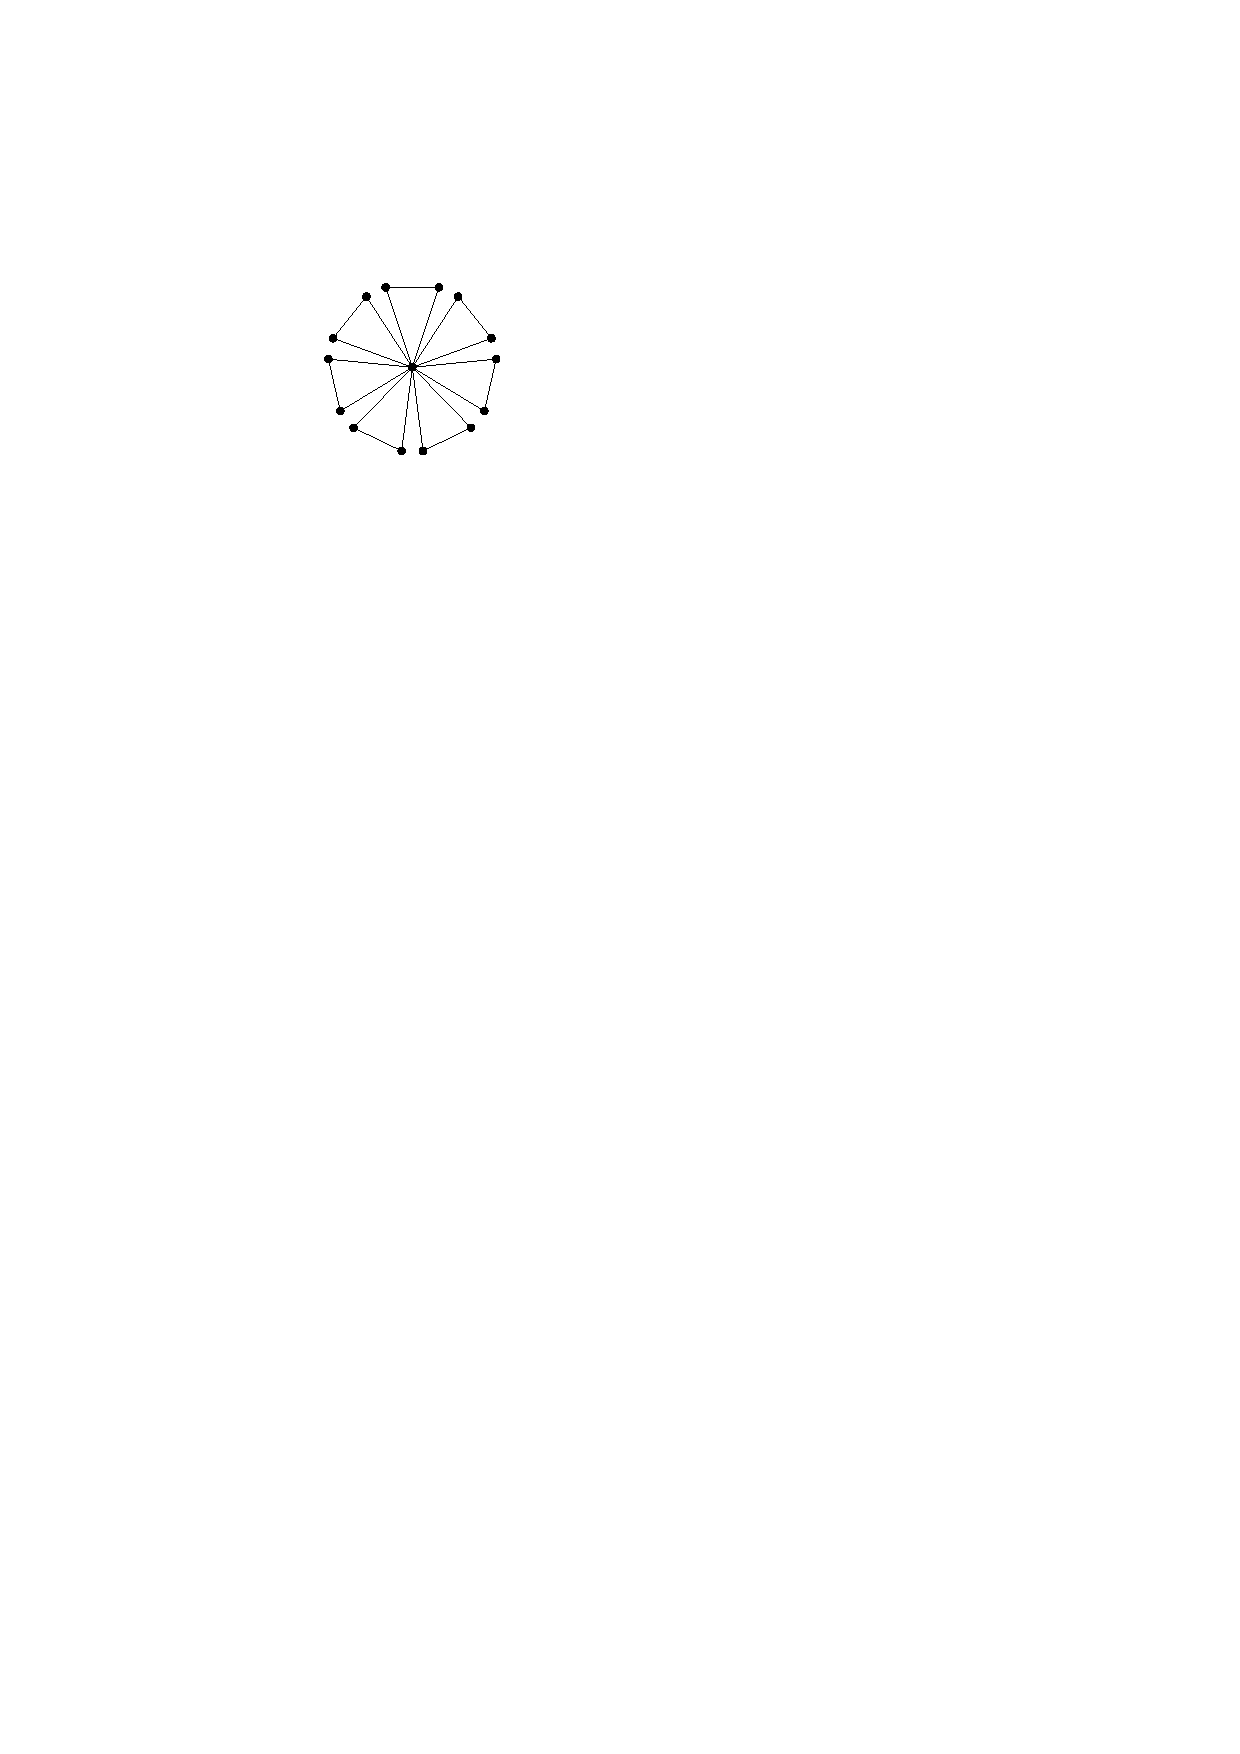
\includegraphics{friendship.pdf}
\end{center}

\dk Nejprve si připomeňme, co jsou to konečné projektivní roviny.

\df Konečná projektivní rovina je množina bodů a přímek, že:
\begin{enumerate}
	\item Každé dvě přímky sdílejí právě jeden bod.
	\item Každé dva body spojuje právě jedna přímka.
	\item Existují 4 body a žádná přímka neprotíná více než dva z nich.
\end{enumerate}

Nyní si označme symbolem $N(v)$ množinu sousedů vrcholu $v$. Všimneme si, že
sousedství pro náš graf přesně odpovídají přímkám v KPR a body jsou body. Protože ale třetí
podmínka by znamenala, že naše věta neplatí, budeme si přát, aby to KPR nebyla
-- pak snadno najdeme vrchol, který je spojený s každým dalším.

Pro spor tedy předpokládejme, že graf KPR je. Protože v KPR mají všechny přímky stejnou mohutnost, je také $d$-regulární. Navíc každé $u,v$ má právě jednoho společného souseda, což znamená, že $G$ je silně regulární s parametry  $e=f=1$.

Podle předchozí věty to ověříme: možnost (a) nastat nemůže, protože $e=f$.
Počítejme tedy, že nastala možnost (b). Protože je to KPR řádu $m$, tak $d=m+1$ a $n=m^2 + m + 1$.
\begin{align}
	(e-f)^2 - 4(f-d) = 0^2 - 4 - 4(m+1))= s^2 \\
	4m = s^2 \\
	s=2\sqrt m 
\end{align}
A ověříme celočíselnost polynomu $p$ s tím, že $t:=s/2=\sqrt m$, tedy $s=2t$ a $m=t^2$:
\begin{align}
	p &= {d \over 2fs} ((d-1+f-e)(s+f-e)-2f) \\
	&= {m+1 \over 4t} ((m+1+0)(2t+0)-2)\\
	&= {(t^2 + 1)(t^3-1) \over 2t}
\end{align}
Což má být přirozené číslo. To je pravda zřejmě jenom pro $t=1$, tedy $n=3$ a pokud náš graf není trojúhelník, jde to spor. Pokud to trojúhelník je, splňuje žádanou vlastnost triviálně. \qed


